\documentclass[12pt]{article}
\usepackage[margin=1.5in]{geometry}
\usepackage{graphicx}
\usepackage{blindtext}%for dummy text
\usepackage{fancyhdr}
\usepackage{nopageno}%removes number on titlepage
\usepackage[parfill]{parskip}%removes indent for new paragraph, adds space between paragraphs

\begin{document}
% Cover page
\author{Evan Pete Walsh\footnote{Mathematics major at St. Lawrence University. I am open to questions and comments and can easily be reached by email at epwalsh@iastate.edu.}}
\title{The Performance of Momentum Investing: Consequences for Market Efficiency, or Not}
\maketitle

\newpage
\begin{abstract}
The efficacy of the momentum strategy of investing in stocks, buying past winners and selling past losers, to produce abnormal returns is often cited as a counter-example for strict market efficiency. However, the advent of momentum mutual funds and exchange traded funds over the past decade has allowed us to analyze the success of actual momentum portfolios, finding that they have significantly underperformed the market. While transaction costs may explain much of the poor performance, the changing market betas and option-like behavior of the portfolios are also a factor, particularly following a prolonged market decline. As a result, it appears that momentum falls short in practice of disproving market efficiency.
\end{abstract}

\newpage

\tableofcontents
 
\newpage
% Fancyhdr
\pagenumbering{arabic}%starts numbering at "1"
\pagestyle{fancy}
\fancyhead[L]{St. Lawrence University}
\rhead{\thepage}
\rfoot{\today}
\cfoot{}%removes default page number at bottom center

\section{Introduction} %%%%%%%%%%%%%%%%%%%%%%%%%%%%%%%%

Momentum in the stock market, the ability of past performance to predict future performance, has been well documented over the past three decades. Research on the subject originated with papers such as De Bondt and Thaler (1985, 1987),\footnote{De Bondt and Thaler (1985, 1987)  proposed that stock prices overreact to information and thus buying past losers and selling past winners would result in abnormally high returns.} who demonstrated that past returns from 3 to 5 years exhibit \emph{negative} correlation with future returns, and Jegadeesh and Titman (1993), who showed that past returns from 3 to 12 months exhibit \emph{positive} correlation with future returns.\footnote{Grinblatt and Moskowitz (2004) find that most of the negative correlation with past 3 year returns and future returns is limited to January, suggesting there may not be a connection between the 3-5 year reversals 12 month momentum.} Further, Jagedeesh (1990), Lo and MacKinaly (1990), and Lehmann (1990) provide evidence for a reversal effect with high past 1 month returns.

The typical equity momentum strategy examined in the literature is the self-financing portfolio that goes long the stocks within the top decile of returns over the past 12 months, less the most recent month, and short the stocks within the bottom decile of returns. Returns from the last month are not considered owing to the 1 month reversal effect. Historically, the exceptional returns of this strategy have not been explained by either the capital asset pricing model (CAPM) or the Fama-French three-factor model, which has inspired a four-factor model to encompass exposure to momentum. This model, proposed by Carhart (1997), is represented by Equation 1.
\begin{equation}
r_{i,t}-r_{f,t}=\alpha_{i}+\beta_{i,m}(r_{m,t}-r_{f,t})+\beta_{i,s}SMB_{t}+\beta_{i,h}HML_{t}+\beta_{i,w}WML_{t}+\epsilon_{t},
\end{equation}
Carhart's model extends the Fama-French three-factor model by adding the $WML_{t}$ term for the difference in return at time $t$ between the $W$inning decile and the $L$osing decile of the past 12 months. As in the three-factor model, $SMB_{t}$ still stands for the returns of $S$mall market cap stocks $M$inus the returns of $B$ig market cap stocks, and $HML_{t}$ for the returns of $H$igh book-to-market value stocks $M$inus $L$ow book-to-market value stocks.

\begin{figure}[p]% separate page
\centering
\caption{\textbf{Log Cumulative Returns - Small Cap.} {\footnotesize This figure displays the cumulative log returns of a portfolio consisting of the top decile of momentum stocks, formed with regard to $t-12$ through $t-2$ months, within the bottom 20\% of market equity, and the cumulative log returns of a benchmark index consisting of all bottom 20\% market equity stocks.}}
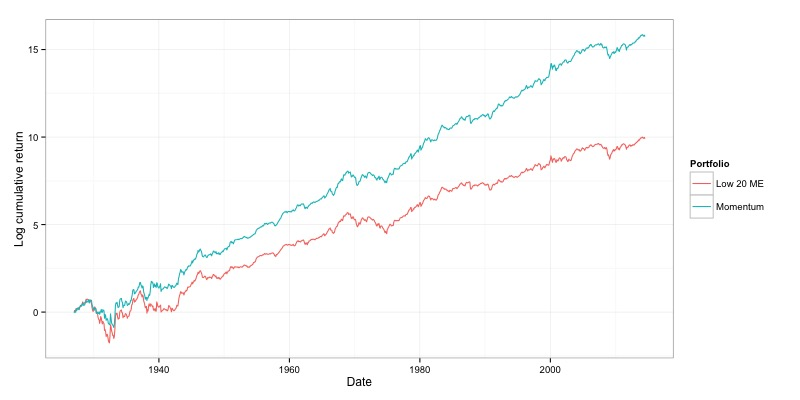
\includegraphics[scale=0.52]{Figures/01-Lo20.JPEG}
\end{figure}
\begin{figure}[p]
\centering
\caption{\textbf{Log Cumulative Returns - Large Cap.} {\footnotesize This figure displays the cumulative log returns of the top decile of momentum stocks of the top 20\% of market equity, and the cumulative log returns of a benchmark index consisting of all top 20\% market equity stocks.}}
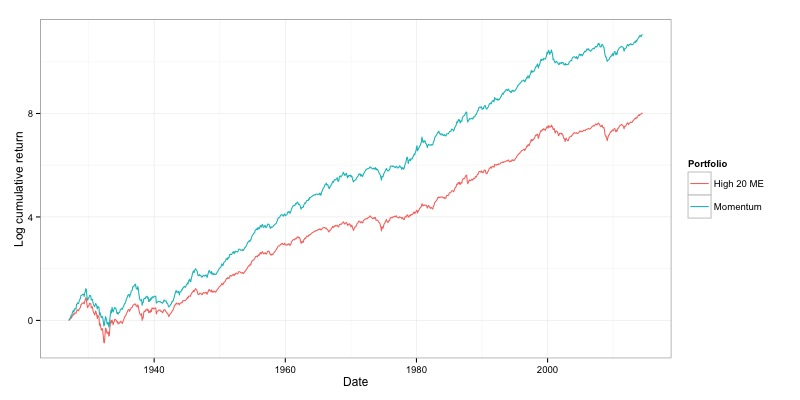
\includegraphics[scale=0.52]{Figures/02-Hi20.JPEG}
\end{figure}

Figures 1 and 2 illustrate how high momentum stocks have historically outperformed stocks of similar market capitalization during our time-table of January 1927 through July 2014.\footnote{Momentum strategies actually performed relatively poorly before WWII.} Table 1 reports the annualized mean return, standard deviation, and alpha (with respect to the three-factor model) of the momentum decile and WML portfolios over this same time period. Portfolio 1 represents the stocks within the lowest decile of returns over the formation period (hence forth referred to as the Low10 portfolio) while portfolio 10 represents those within the highest (referred to as the High10 portfolio). The annual return spread between the top and bottom deciles for momentum was an average of 14.3\%, with an annualized alpha of 7.7\% for the top decile, and 17.7\% for the WML portfolio. 

\begin{table}[h]
\centering
\caption{\textbf{Summary of Momentum Portfolios, 1927-2013} {\footnotesize This table reports the annualized mean return (\%), standard deviation, and alpha with respect to the three-factor model for momentum decile portfolios during the period from January 1927 to July 2014. }}
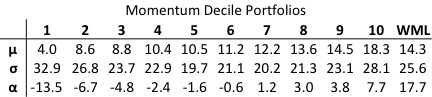
\includegraphics[scale=0.6]{Deciles.jpg}
\end{table}

Clearly, momentum appears to contradict strict market efficiency in which, according to Fama (1991), ``security prices fully reflect all available information." If strong (weak) past performance is an indication of future strong (weak) performance, then investors should buy (short) the winning (losing) firms today, causing their prices to rise (fall) now to where momentum predicts them to be in, say, a year from now.\footnote{Not taking into account the time-value of money.} Thus, if past performance contains information about future performance, then that information should already be reflected in the price, yet the persistence of momentum suggests otherwise.

Of course, the feasibility of this strategy comes into question due to the high turnover rate of the portfolio, which undoubtedly racks up high transactions costs.\footnote{Despite the high transaction costs fundamental to momentum strategies, there are actually some favorable tax implications to such a strategy. Namely, the consistent selling of losing stocks leads to realized capital loses that may be used to offset capital gains taxes. For more on the role of taxes with momentum, see Grinblatt and Moskowitz (2004).} Indeed, while round-trip trading costs for the winner and loser portfolios during each new formation period were assumed to be around 2\% each in early studies, Li, Brooks, and Miffre (2009) estimate the costs to be closer to 3.77\% for the winners and 6.71\% for the losers. The theoretical momentum portfolios rebalance monthly, which, depending on the turnover rate, would incur substantial transaction costs. 

Nevertheless, the popularity of momentum investing has resulted in several mutual funds and exchange traded funds (ETFs) over the past decade that attempt to capture momentum through variations of the strategy. This has given us the opportunity to study the performance of real momentum portfolios, in particular the AQR Momentum Fund (AMOMX), Bridgeway Small Cap Momentum Fund (BRSMX), Rydex SGI Long Short Momentum Fund (RYAMX), and the PowerShares DWA Momentum Portfolio (PDP).

We find that each of these funds have significantly underperformed the market since their respective date of inception to July 7, 2013, while our theoretical momentum portfolios have significantly outperformed the market. The AMOMX, PDP, and RYAMX all exhibit statistically significant negative alphas.\footnote{The BRSMX's alpha is not significantly different from 0.} From July 9, 2009 to July 7, 2013, the compound annual growth rate (CAGR) of the AMOMX was 12.29\%, with an annualized alpha of -7.44 and Sharpe ratio of 0.04. Meanwhile, the theoretical High10 portfolio, unfettered by transaction costs, performed with an alpha of 9.70 and a CAGR of 23.28\% over this same time period. 

Interestingly, all four funds except the BRSMX have outperformed the WML portfolio. However, because their cumulative returns are closer to the WML than the High10, we attempt to characterize the strategies of each fund by seeing how much exposure they have to Low10 and High10 portfolios. If we see significant negative correlation with the Low10 portfolio, then we can conclude that these funds are shorting the many of the same stocks as the WML portfolio. To do this, we run regressions with the returns of the AMOMX, BRSMX, PDP, and RYAMX as the dependent variables, and the Low10 and High10 returns as the predictors. We find that each of these funds have small but significant \emph{positive} correlation with the Low10 portfolio, but much greater positive correlation with the High10 portfolio. Our conclusion is that these funds favor long strategies. Consequently, the funds also have negative correlation with the WML portfolio.

To investigate the impact of transaction costs on these funds, we implement a modified form of the four-factor model with the High10 as a predictor instead of the WML term.\footnote{We substitute the High10 for the WML as a predictor since the funds have negative correlation with the WML portfolio, but strong positive correlation with the High10, meaning that their strategies are closer to that of the High10.} If the strategies of these funds are similar enough to that of the High10, then the intercepts of these regressions should give us an idea of the magnitude of transaction costs (assuming the intercept is negative). We do see significantly negative intercepts for all four funds, the mildest of which is -7.401 for the AMOMX. This means that the AMOMX incurs roughly 7.4\% per year in transaction costs.

Another cause for the poor performance may be due to changing market betas of momentum portfolios, particularly following periods of prolonged or dramatic market decline and high volatility. Consistent with Daniel and Moskowitz (DM) (2011), we find that the WML portfolio tends to load up on stocks with low market betas during a bear market, while shorting stocks with high market betas. This makes sense since we would expect high beta stocks to sharply drop in price as the market declines, thus putting them in the loser group, and low beta stocks to suffer less, thereby putting them in the winner group. Then, as the market rebounds, the portfolio is short high beta stocks, which perform well as the market rises, and long low beta stocks, which perform poorly as the market rises. 

We estimate that when the cumulative return of the market over the previous two years was negative (i.e. a bear market), the market beta of the High10 portfolio is, on average, 0.335 lower than when the past two year cumulative return was positive (i.e. a bull market). Similarly, we expect the beta of the WML portfolio to be an average of 0.913 lower with a bear market, while the beta of the Low10 portfolio tends to be 0.579 \emph{higher} with a bear market. 

The negative correlation between the betas of the High10 and Low10 portfolios is striking as well, especially after major market declines. For instance, during the period from 1999 to 2010, the correlation between the betas of the two portfolios was -0.688, and in the months following the financial crisis of 2008, from March, 2009, to December, 2010, the correlation was -0.953.

We find that the estimated daily market betas of the AMOMX, BRSMX, RYAMX, and PDP follow the daily beta of the High10 very closely, exhibiting the same behavior after market declines. The beta for RYAMX, for example, peaked above 2.0 before the crisis of 2008, since the market was at an all-time high, but then fell below 1.0 a year later when the market had hit a low point around February of 2009. Overall, since the RYAMX began on June 21, 2005, we find that its beta is on average 0.177 higher during a bull market. Similarly, since the PDP began on March 1, 2007, its beta is on average 0.128 higher during a bull market.\footnote{The RYAMX and PDP are the only momentum portfolios with which we have data going back to before the financial crisis of 2008.}

Upon further investigation, we find that during a bear market, when the contemporaneous return of the market is positive, the betas of the RYAMX and PDP are -0.200 and -0.294 lower, respectively, than when the contemporaneous return of the market is negative.\footnote{DM find that the difference between up- and down-market betas during bear markets for the WML portfolio is mostly driven by the loser group.} This suggests that these funds demonstrate option-like behavior in regards to the market. Specifically, the portfolios are essentially ``short a call option on the market," according to DM. The optionality we find in the RYAMX and PDP is not as strong as in the WML portfolio, however, which is not surprising since DM find that most of this optionality is driven by the Low10 portfolio. 

While we have verified empirically that the changing market betas of several real momentum portfolios has an effect on their performance relative to the market, the only explanation for why these funds have considerably underperformed the theoretical momentum portfolios is transaction costs. All together, it appears that momentum falls short of disproving stock market efficiency when the cost of trading is considered. 

This paper will proceed as follows: Section 2 provides a brief overview of the literature most referenced in our study. Section 3 describes the sources of our data and the methodology for creating our portfolios. Section 4 reports the performance of our momentum strategies in raw return and with regard to alphas and Sharpe ratios and provides a method for estimating the transaction costs. In Section 5, we analyze the changing market betas of different momentum portfolios and how these affect their performance, and in Section 6 we conclude and offer ideas for further research.

\section{Literature Review} %%%%%%%%%%%%%%%%%%%%%%%%%%%%%%%%%%%%%

Although numerous papers report the efficacy of momentum to produce abnormal returns, most of them do not properly account for transaction costs. According to Lesmond, Schill, and Zhou (LSZ) (2004), these studies underestimate the transaction costs associated with momentum strategies because they only consider the trading of large and liquid stocks. Yet, a considerable proportion of the profits from momentum strategies are generated from selling the losers, which generally have lower market cap, price, and liquidity. 

LSZ focus on a WML momentum strategy with a 6-month formation and holding period, and find that the returns generated do not make up for the transaction costs. However, their study falls short in assessing the WML strategy with different formation and holding periods. Their investigation only finds that the returns of a strategy that rebalances \emph{twice} a year are not significant considering the trading costs, yet a portfolio that rebalances only once a year, i.e. a 12-month holding period, will theoretically incur half of the yearly transaction costs and thus may still produce abnormal returns beyond the costs of rebalancing.\footnote{In practice, the transaction costs will probably not be half as much for the 12-month portfolio since some of the stocks included during a holding period of the 6-month portfolio may still be included in the next holding period, therefore not adding anymore costs.}

Li, Brooks, and Miffre (LBM) (2009) expand upon LSZ by investigating the impact of transaction costs on portfolios with combinations of holding and formation periods of 3, 6, and 12 months in the UK. They find that when they assume full portfolio turnover, only strategies with 12-month holding periods still exhibit significant abnormal returns. Yet, when they consider actual turnover, which is often around 70\%, they find that a total of ``6 out of 9 momentum strategies generate significant net momentum profits at the 5\% level." 

\subsection{The Higher Transaction Costs of the Losing Portfolio}

Whether or not the conclusions made by LBM remain true in US markets will be a subject of further study. However, given the poor performance of momentum funds compared to the theoretical portfolios to date, it is evident that trading costs have a greater impact than previously assumed in the literature.

As mentioned before, much of the costs incurred come from the asymmetry in the price of selling the losers versus buying the winners, due to the tendency of the losers to be smaller and less liquid. From 1926 to 2013, the mean percent difference in market cap of stocks in the highest and lowest momentum deciles was 16\%, with a standard deviation of 1.42\%. That is, the ME of the bottom decile of momentum stocks was an average of 16\% lower than the ME of the top decile.

It is unclear if the lower ME and liquidity of the loser stocks are the sole reasons for the asymmetry in transaction costs. Yet the result is, at least in the UK, that transaction costs for selling the losers are about twice as much as that for buying the winners. This may partly explain why some of the mutual funds and ETFs that we study employ long-side-only tactics to capture momentum. 

\subsection{Momentum Crashes}

Another reason that may explain why funds stick to long-side-only tactics is the susceptibility of the losing stocks to reverse and gain rapidly following periods of market decline, resulting in dramatic crashes to the WML portfolio. DM and Grundy and Martin (GM) (2001) provide excellent insight into this matter with their studies of the variation in the beta of the momentum portfolio over different market conditions.

In agreement with their findings, we see that the WML strategy with a 12-month formation period tends to load up on stocks with low market betas during prolonged market declines, and go short stocks with high market betas.\footnote{DM find that the the beta for the lowest decile of momentum stocks (i.e. the ones that the portfolio shorts) rises above 3 following market declines, while the betas of the highest decile falls below 0.5.} This explains why the short position stocks tend to do very well as the market rebounds, and the stocks that the portfolio is long tend to perform relatively poorly.

GM, however, propose that the performance of the momentum strategy can be substantially improved, particularly through crash periods, by dynamic hedging of market and size risk. Unfortunately, their method is not actually implementable since their hedging coefficients are calculated using betas that are measured on future returns. Nevertheless, as DM note, ``while not technically valid, [their procedure] should not bias their estimated performance if their forward-looking betas are uncorrelated with future market returns." Yet DM find a strong correlation of the market to the beta of the loser portfolio by calculating up- and down-market betas. 

Consistent with Henriksson and Merton (1981), the up-beta is calculated using data only from when the contemporaneous return of the market was positive, and the down-beta using data only from when the contemporaneous return of the market was negative. DM find that, in a bear market, the loser ``momentum portfolio up-market beta is more than double its down-market beta ($-1.47$ versus $-0.66$), and that this difference is highly statistically significant."\footnote{DM also note that, ``Outside of bear markets, there is no statistically significant difference" between the up- and down-market betas of the loser portfolio.}

We extend the research done by DM and GM by examining how the market betas of several different momentum funds have varied since each fund's inception, particularly with regard to the market crash following the events of 2008. We find that the betas of the AMOMX, BRSMX, RYAMX, and PDP follow the betas of the High10 portfolio very closely. Further, the betas of the RYAMX and PDP exhibit similar correlation with the return of the market as the WML beta.

\section{Data Description and Methodology} %%%%%%%%%%%%%%%%%%%%%%%%%%%%%

Our primary data source for our theoretical portfolios is Ken French's data library,\footnote{$http://mba.tuck.dartmouth.edu/pages/faculty/ken.french/data_library.html$. Ken French is a professor of finance at Dartmouth College. His whose work with Eugene Fama on the value effect and the three-factor model has been invaluable to the finance community.} which uses all US CRSP firms listed on the NYSE, AMEX, and NASDAQ with a valid price and market equity and a share code of either 10 or 11. 

Momentum portfolios are broken into ten groups as determined by monthly NYSE prior return decile breakpoints.\footnote{Note that while firms from the NYSE, AMEX, and NASDAQ are all considered, breakpoints are only based on the NYSE. According to DM, the result of this is generally putting more firms in the bottom and top momentum portfolios since the variance of returns for the AMEX and NASDAQ is greater than that of the NYSE.} Returns are considered only for the past 12 months, not counting the most recent month. The holding period for each portfolio is 1 month, after which rebalancing occurs according to the same breakpoints. We often reference the High10 portfolio, which is the top momentum portfolio. The High10 is composed of the stocks representing the highest decile of returns. Conversely, the Low10 is the bottom momentum portfolio, which is composed of the stocks representing the lowest decile of returns. Returns of the WML portfolio are calculated as the return of the High10 at time $t$ minus the return of the Low10.

Alphas are calculated with respect to the Fama-French three factor model. The market return and risk free rate, as well as returns for the SMB and HML portfolios also come from Ken French's data library. The market return is based on the CRSP value weighted index, while the risk free rate is the 1-month Treasury-bill rate from Ibbotson Associates. The SMB and HML portfolios are rebalanced every 6 months. Returns of the small minus big portfolio are calculated by taking the mean return of three small portfolios, representing small value, neutral, and growth stocks, minus the mean return of three large portfolios defined in the same way. Conversely, returns of the high minus low portfolio are calculated by taking the mean return of two value portfolios, representing small and big \emph{value} stocks, minus the mean returns of two growth portfolios, representing small and big \emph{growth} stocks.

Historical data for the AMOMX, BRSMX, RYAMX, and PDP come from the database of TradeKing Group, Inc. Due to the fact that momentum funds are a somewhat recent phenomenon, the largest dataset that we have only goes back to 2005.

All statistical analysis was done using R.

\section{Momentum Funds} %%%%%%%%%%%%%%%%%%%%%%%%%%%%%%%%%

Although momentum has been well studied for three decades now, momentum style mutual funds, ETFs, and indices are a recent phenomenon. The longest standing mutual fund that we investigate is the RYAMX, founded in 2005, which is one of the few momentum funds to employ a short strategy.\footnote{Out of the the 12 funds and indices we have investigated, the RYAMX is the only one that explicitly shorts low momentum stocks.} A summary of several of the major momentum funds and indices available today is shown in Figure 3, with a brief description of their variation of the strategy, including how often the portfolio is reconstituted and how each asset is weighted.

Several of the funds and indices explicitly rebalance no more than 4 times a year, and widen their long stock selections to approximately the top third of returning stocks. In fact, none of these portfolios follow the exact strategy of either the WML or High10.

\begin{figure}[p]
\caption{\textbf{Summary of Selected Momentum Funds and Indices.}}
\centering
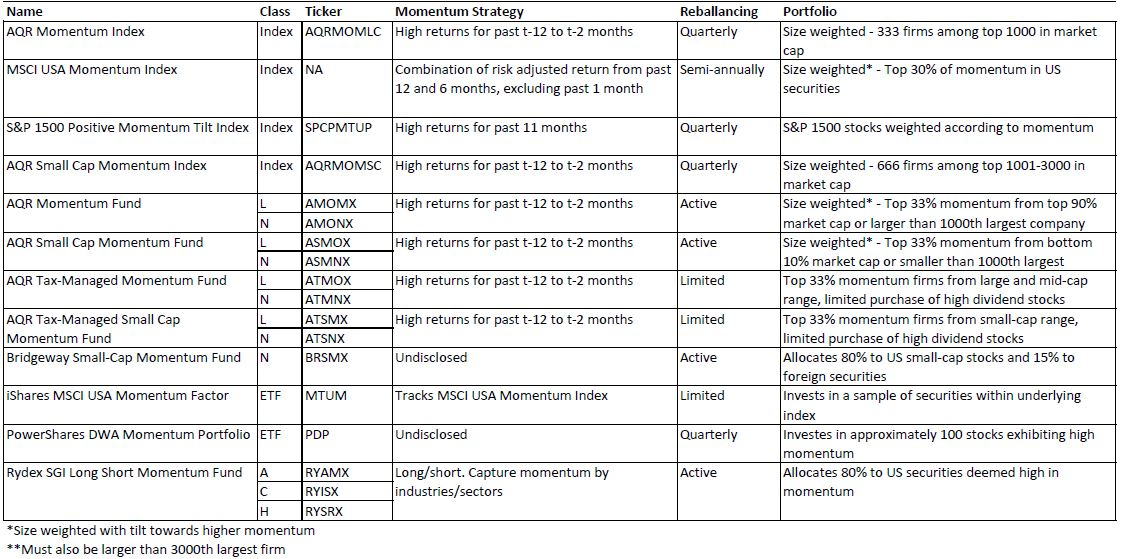
\includegraphics[angle=270, scale=0.65]{SummaryOfFundsIndices.jpg}
\end{figure}

As far as the funds that disclose their methods, the strategies closest to that of the High10 are employed by AQR Capital Management,\footnote{The founder of AQR Capital Management, Clifford Asness, has contributed substantially to the research on momentum. Several of his papers are listed as references here.} specifically the AMOMX. The AMOMX rates stocks based on their returns for the past 12 months, excluding the most recent month, and then weights each security based on size with a tilt towards higher momentum stocks. In general, their strategy has been to invest in stocks within the top 33\% of returns over the ranking period that are within the top 90\% of market cap. 

The similarities of the AMOMX's strategy to that of the High10 are illustrated by comparing estimated market betas. Figure 13 shows that from January 2010 to March 2012 the betas for the two portfolios almost track each other exactly, providing evidence that their portfolios have significant overlap, or simply hold stocks with very similar market betas. It is unclear what caused the divergence in betas from March 2012 onward, or whether this asymmetry will continue. Perhaps this marks a change in the strategy of the AMOMX.

\subsection{Performance}

To evaluate the performance of 3 mutual funds and an ETF that employ momentum strategies, we find their mean return and standard deviation (less the risk-free rate), Sharpe ratios, and alphas along with the test statistics and p-values. Alphas are calculated with respect to the Fama-French three factor model, as shown in Equation 2, in order to capture any potential exposure to the size and value factors.

\begin{equation}
r_{i,t}-r_{f,t}=\alpha_{i}+\beta_{i,m}(r_{m,t}-r_{f,t})+\beta_{i,s}SMB_{t}+\beta_{i,h}HML_{t}+\epsilon_{t},
\end{equation}

Table 2 reports these statistics from the inception date of the fund to July 31, 2013. 

\begin{table}[h]
\centering
\caption{\textbf{Performance of Selected Momentum Funds and Indices Since Inception.} {\footnotesize This table summarizes the returns of 4 selected momentum funds that are available to non-institutional investors. Mean returns and alphas are annualized. Alphas are with respect to the Fama-French three factor model. Test statistics and p-values are reported for the alphas. The data for each fund/index goes back the date listed in the ``Date" column.}}
\begin{tabular}{l | l | c | c | c | c | c | c}
\hline
Ticker & Date & $\mu_{R_{i,t}-R_{rf,t}} $ & $ \sigma_{R_{i,t}-R_{rf,t}} $ & SR & $\alpha$ & t.s. & P\\
\hline
AMOMX & 7/9/09 & 14.11 & 1.27 & 0.04 & -7.44 & -2.928 & 0.003 \\
BRSMX & 5/24/10 & 5.04 & 1.66 & 0.01 & -5.22 & -0.403 & 0.687 \\
PDP & 3/1/07 & 1.49 & 1.65 & 0.00 & -7.84 & -2.294 & 0.022 \\
RYAMX & 6/21/05 & 0.13 & 1.40 & 0.00 & -8.69 & -2.525 & 0.012 \\
\end{tabular}
\end{table}

\begin{figure}[p]
\centering
\caption{\textbf{Comparisons of Cumulative Return: AMOMX and BRSMX.}}
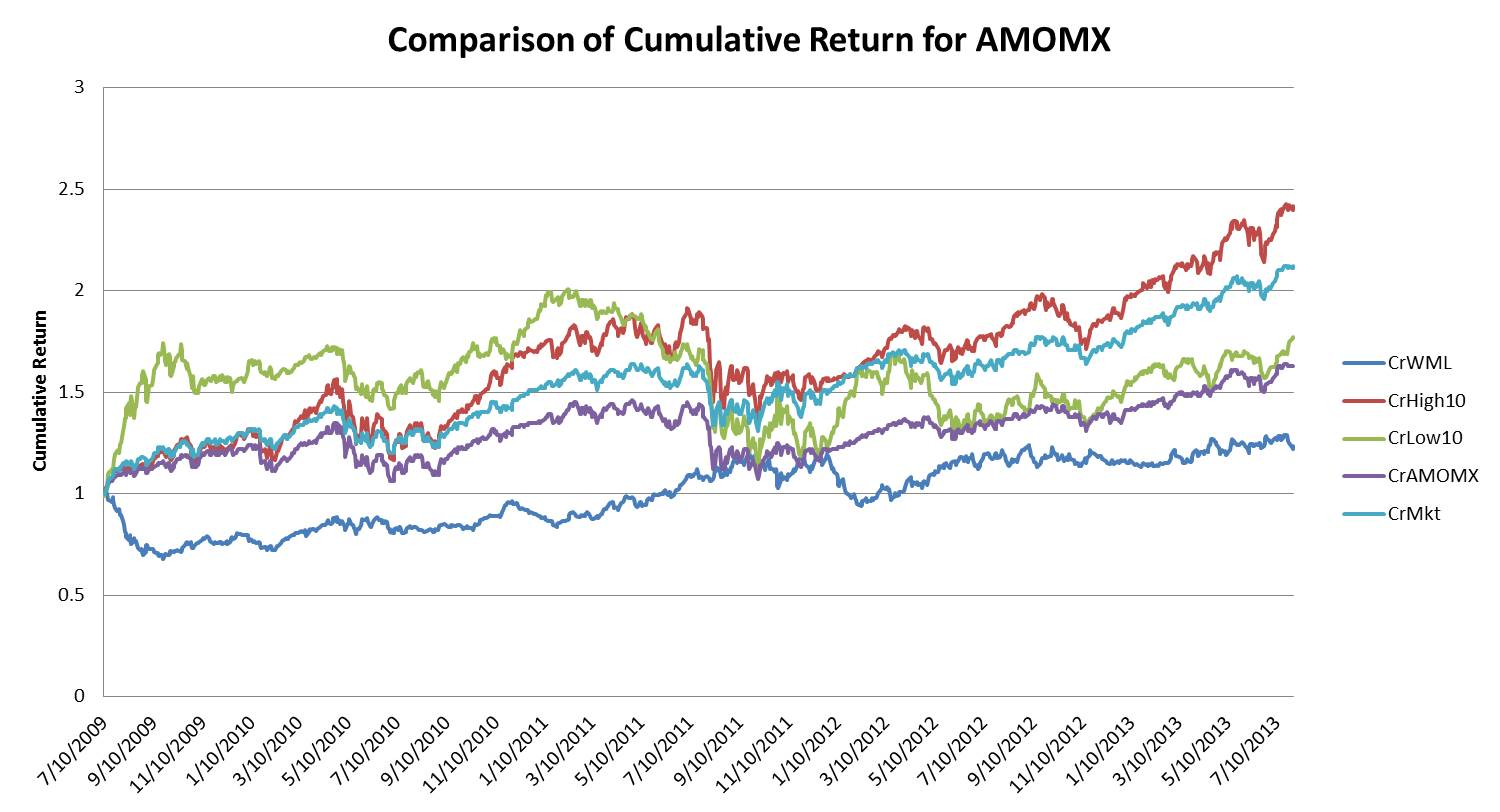
\includegraphics[scale=0.6]{CompAMOMX.jpg}
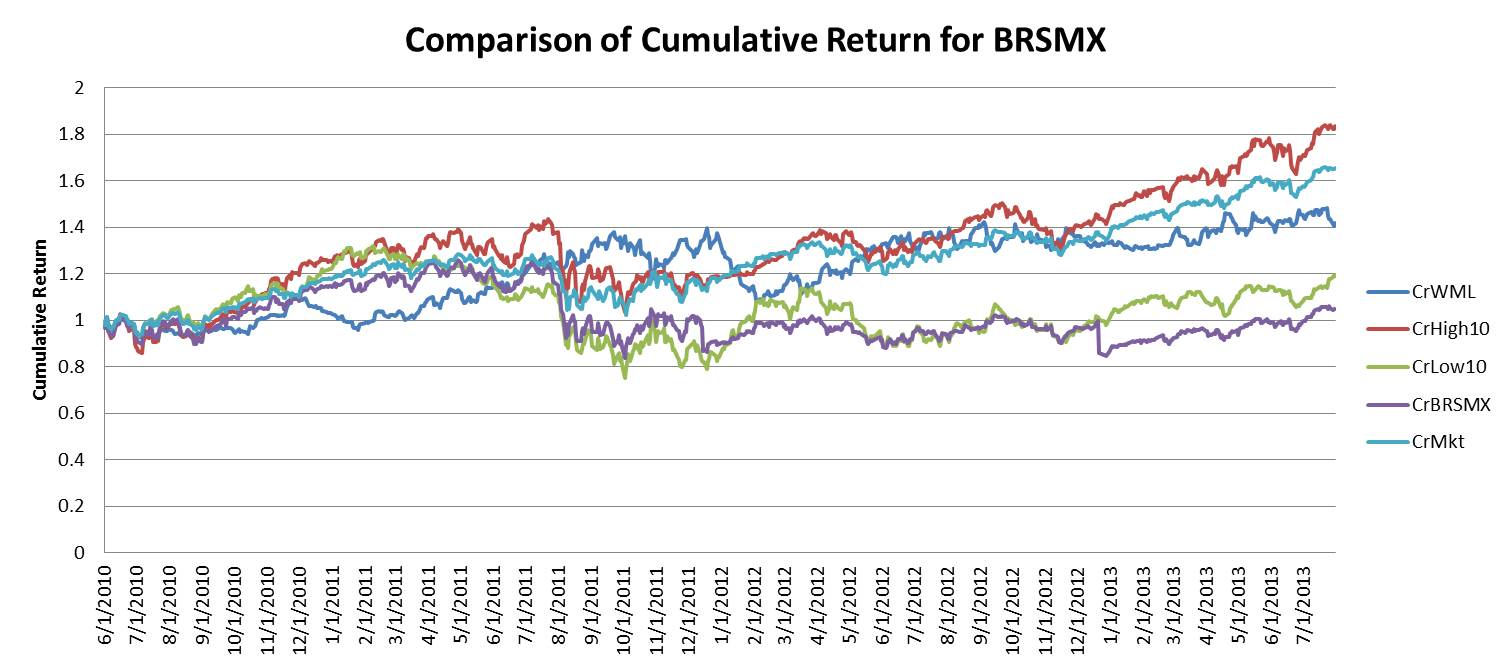
\includegraphics[scale=0.6]{CompBRSMX.jpg}
\end{figure}

\begin{figure}[p]
\centering
\caption{\textbf{Comparison of Cumulative Return: PDP and RYAMX.}}
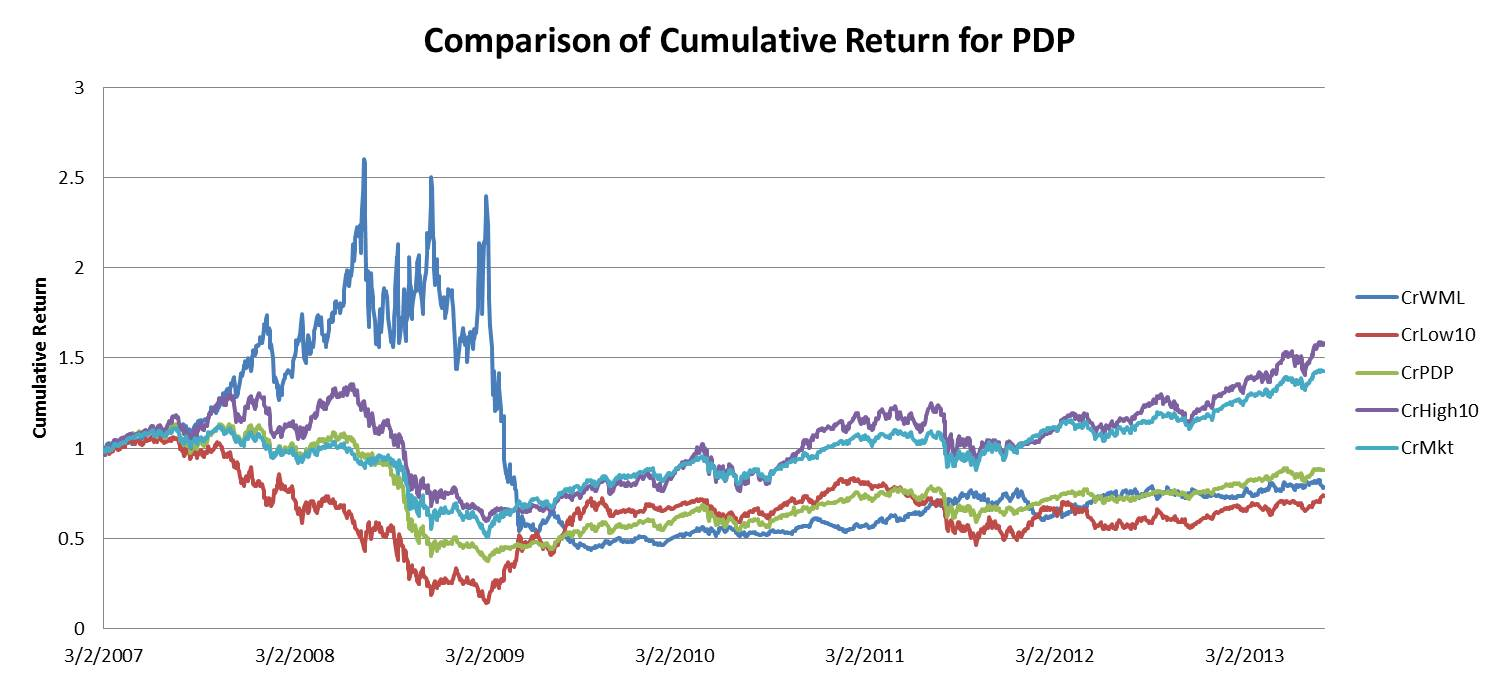
\includegraphics[scale=0.6]{CompPDP.jpg}
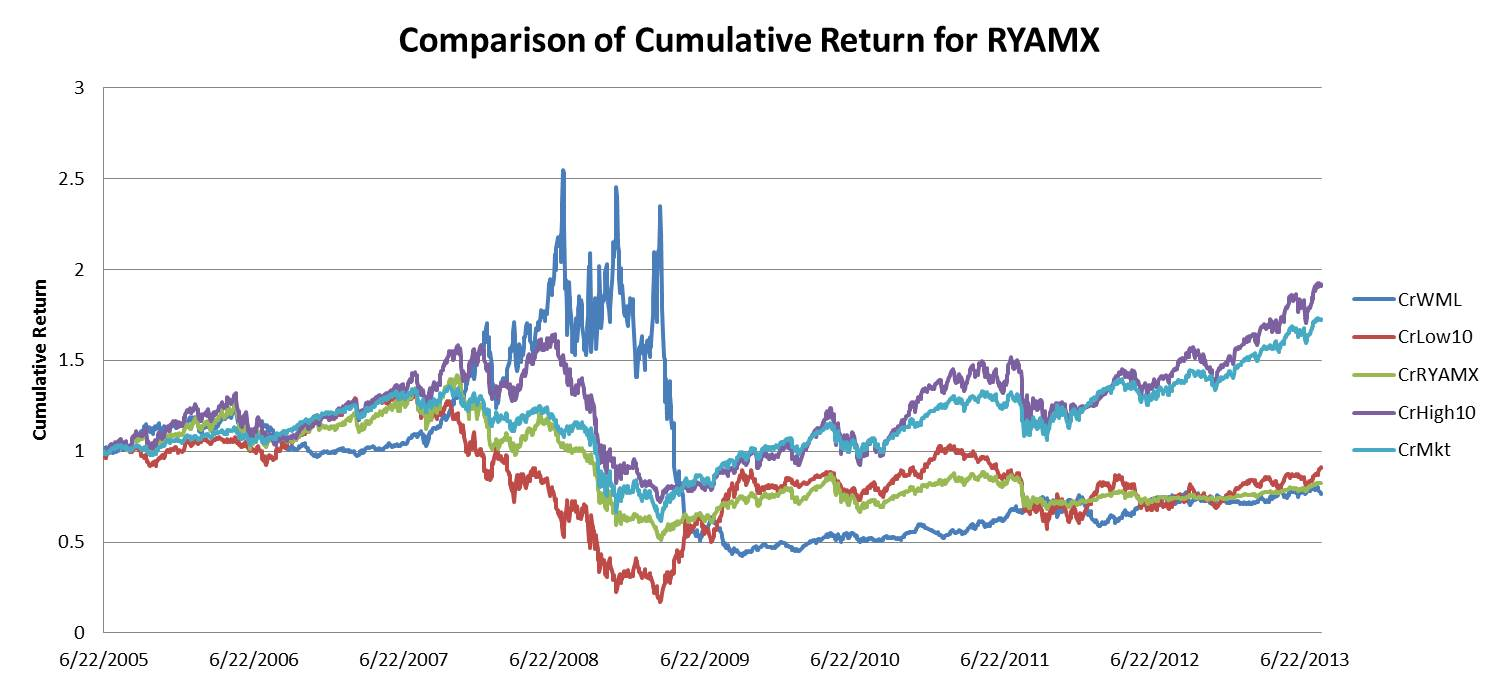
\includegraphics[scale=0.6]{CompRYAMX.jpg}
\end{figure}

As shown above, returns have not been impressive for all four portfolios. We find negative alphas for each portfolio, which are significant at the 0.05 level for the AMOMX, PDP, and RYAMX. The alpha for the BRSMX is not significantly different from 0. Meanwhile, the transaction cost free High10 strategy has performed with an annualized alpha of 9.70 since 2009, 1.24 since 2007, and 1.56 since 2005. Indeed, transaction costs appear to have very serious consequences on the efficacy of the momentum strategy.

Figures 4 and 5 compare the cumulative return of the market, High10, Low10, and WML to the AMOMX, BRSMX, PDP, and RYAMX. All four fund perform below the market and High10, yet the AMOMX, PDP, and RYAMX succeed at surpassing the WML, although not by much.

\subsection{Characterizing the Strategies of Momentum Funds}

Since the cumulative returns of the AMOMX, PDP, BRSMX, and RYAMX are much closer to that of the WML than the High10, we would like to determine how much exposure they have to shorting the loser group. To do this, we run regressions with the Low10 and High10 as predictors for the returns of each fund. Equation 3 shows the form of the model, where $L_{t}$ is the returns of the Low10 portfolio for day $t$, and $W_{t}$ is the returns of the High10.

\begin{equation}
r_{i,t}=\alpha_{i}+\beta_{i,L}L_{t}+\beta_{i,H}W_{t}+\epsilon_{t}
\end{equation}

The AMOMX explicitly only goes long high momentum stocks, so we expect to see a large positive $\beta_{H}$ coefficient and a $\beta_{L}$ coefficient that is not significantly different from 0. For the other funds, if they engage in any substantial short selling then we expect to see a negative $\beta_{i,L}$ coefficient. Table 3 reports the estimated coefficients.

\begin{table}[h]
\centering
\caption{\textbf{Results of Regression 3.} \footnotesize{Test statistics and p-values (in parenthesis) are reported below the estimated coefficients.}}
\begin{tabular}{l | c | c | c }
\hline
Fund & $\alpha_{i}$ & $\beta_{i,L}$ & $\beta_{i,H}$ \\
\hline
AMOMX & -0.019 & 0.128 & 0.675 \\
 & -1.854 (0.064) & 14.407 ($\approx 0$) & 68.126 ($\approx 0$) \\
\hline
BRSMX & -0.050 & 0.355 & 0.649 \\
 & -1.863 (0.063) & 15.366 ($\approx 0$) & 24.352 ($\approx 0$) \\
\hline
PDP & -0.029 & 0.160 & 0.709 \\
 & -2.283 (0.023) & 30.425 ($\approx 0$) & 76.005 ($\approx 0$) \\
\hline
RYAMX & -0.033 & 0.108 & 0.670 \\
 & -2.851 (0.004) & 20.270 ($\approx 0$) & 74.878 ($\approx 0$) \\
\end{tabular}
\end{table}

Surprisingly, every fund including the AMOMX has a significantly positive $\beta_{i,L}$ coefficient, when we expect it to be negative or zero. However, the $\beta_{i,H}$ coefficients are significantly positive and relatively large (greater than 0.5), which leads to the conclusion that each of the funds favor long strategies. It also demonstrates that if the managers of these funds are shorting stocks, they are not choosing the same stocks as those in the Low10. Perhaps they use a shorter formation period.

\subsection{Estimating Transaction Costs}

If the strategies of these four funds primarily involve buying the highest momentum stocks, then by comparing their returns to that of the High10, we should be able to roughly estimate the magnitude of the transaction costs. To do this, we modify the Carhart four-factor model by replacing the $WML_{t}$ term with the returns of the High10, $W_{t}$. Thus, our regression is of the form
\begin{equation}
r_{i,t}-r_{f,t}=\alpha_{i}+\beta_{i,m}(r_{m,t}-r_{f,t})+\beta_{i,s}SMB_{t}+\beta_{i,h}HML_{t}+\beta_{i,H}W_{t}+\epsilon_{t}
\end{equation}
Table 4 reports the estimated intercept or alpha, $\alpha_{i}$, from the model. We see that all of the alphas are significantly negative at the 0.05 level except for the BRSMX (P$(\alpha_{i}\neq 0)=0.056$). Hence, we believe that the annual transaction costs incurred by the AMOMX are about 7.4\%, 14.4\% for the BRSMX, 8.7\% for the PDP, and 10.2\% for the RYAMX.

\begin{table}[h]
\centering
\caption{\textbf{Estimated Intercept from Modified Four-Factor Model.} \footnotesize{The estimated intercept, $\alpha_{i}$, is annualized. Test statistics and p-values are reported.}}
\begin{tabular}{l | c | c | c}
\hline
Fund & $\alpha$ & t.s. & p-value \\
\hline
AMOMX & -7.401 & -3.937 & $\approx 0$ \\
BRSMX & -14.401 & -1.912 & 0.056 \\ 
PDP & -8.697 & -3.171 & 0.002 \\
RYAMX & -10.188 & -3.696 & 0.0002 \\
\end{tabular}
\end{table}

While we still do not know the exact magnitude of the transaction costs for these momentum strategies, the impact is clear. Not a single one of these funds has outperformed the market since inception. So, even though momentum may contradict strict market efficiency, the poor performance of these funds is evidence that transaction costs are a vehicle for inefficiencies. In other words, the transaction costs associated with implementing a momentum-style fund serve as a barrier for arbitrageurs to exploit such a strategy.

\section{Analysis of Market Betas} %%%%%%%%%%%%%%%%%%%%%%%%%%%%%

While transaction costs may explain most of the poor performance in the four momentum funds we have studied, the changing market betas may also be a factor. The variation in the market betas of momentum portfolios is most important when examining the crash periods of the momentum strategy, which occur following prolonged market declines. There have been a number of such crashes since 1926, during which the High10 portfolio performs poorly relative to the market, and the Low10 performs well. Specifically, two of the worst durations for the momentum strategy are from the Great Depression up until the end of WWII and in the year following the 2008 financial crisis. From June 1932 through December 1945, the High10 portfolio produced a cumulative gain of only \$3.70 for each dollar invested, while the Low10 gained an outstanding \$26.63. From March 9, 2009 through December 31, 2010, the High10 only gained \$1.85 while the Low10 gained \$5.54 for each dollar invested, according to DM.

Overall, from January 1927 to December 2010, the 11 worst months for momentum returns have come when the past 2-year cumulative market return has been negative. Thus, DM suggest that the changing betas of the momentum portfolios may explain their poor returns over these periods.

Consistent with DM, we estimate the daily market betas using 126 day (approximately 6-month) rolling regressions of the form
\begin{equation}
r_{i,t}=\alpha_{i}+\beta_{i,0}r_{m,t}+\beta_{i,1}r_{m,t-1}+...+\beta_{i,10}r_{m,t-10}+\epsilon_{t},
\end{equation}
where $r_{m,t}$ is the return of the market (CRSP value-weighted index) at day $t$, and $r_{m,t-1}, r_{m,t-2},...,r_{m,t-10}$ are the ten daily lags of the market return, used to account for the lead-lag effects between the market return and the portfolio return. We know this lead-lag effect is present and strong because of the significance of the lagged coefficients, which are particularly strong for the Low10 portfolio and in the 1932 through 1945 era. The estimated market beta is then calculated as the sum of all betas: \[\beta_{i}=\sum_{j=0}^{10}\beta_{i,j}.\]

\subsection{The Crisis of 2008 and Momentum Betas}

Figure 6 is a time series plot of the estimated market betas for the High10 and Low10 portfolios during the period of March 9, 2009 through December 31, 2010. We see that the beta for the High10 portfolio starts off below the beta for the Low10 portfolio. This is intuitive given that the market hit a low on March 9, 2009 with the past 2-year returns of the market being strongly negative, which means that the formation period of the portfolios was during a persistent bear market. Thus, the firms that performed the best, the ones considered in the top decile of returners, were most likely low-beta stocks. Conversely, the firms that performed the worst through the bear market were most likely high beta stocks.

\begin{figure}[h] % [t] to position at top of page
\centering
\caption{\textbf{Estimated Market Betas From Mar, 2009 to Dec, 2010.} {\footnotesize Daily market betas are estimated using rolling 126 day ($\approx6$ month) regressions with 10 daily lags of market return for predictors. In this figure we compare the estimated betas for the highest decile of momentum stocks and the lowest decile.}}
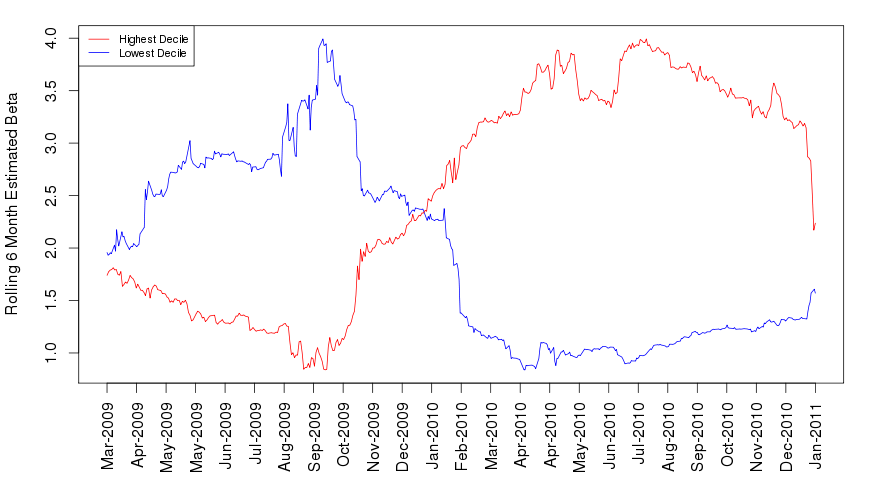
\includegraphics[scale=0.45]{betas2009.png}
\end{figure}

For example, DM find that:

{\footnotesize``...as of the beginning of March 2009, the firms in the loser decile portfolio were, on average, down from their peak by 84\%. These firms included the firms that were hit hardest in the financial crisis: among them Citigroup, Bank of America, Ford, GM, and International Paper (which was levered). In contrast, the past-winner portfolio was comprised of defensive or counter-cyclical firms like Autozone."}

We also notice that within about 9-10 months, as the market was rebounding, the betas of the High10 overtake the betas of the Low10. By May 2010 the cumulative return of the market over the past year, i.e. the formation period of the momentum portfolios, was strongly positive. Hence, it's not surprising that the High10 portfolio contained stocks with relatively high betas and the Low10 with relatively low betas.

Figures 9 gives us a broader view of how the betas of the momentum portfolios have varied from January 1999 to December 2010. Viewed separately, the betas of each portfolio look like a random walk. However, when viewed together, there is a clear negative correlation between the betas of each portfolio: when the High10 betas are low, the Low10 betas are high, and vice versa. In fact, the correlation during this period of the estimated market betas for the High10 and Low10 portfolios was -0.668, while from March 2009 to December 2010, the correlation was -0.953. Similar trends are seen with Figure 7, which shows the estimated betas of the momentum portfolios from January 1932 to December 1945.

Figures 8 and 10 show the estimated market betas for the WML portfolio for the same time periods. We see that the WML beta drops past -3 in the later months of 2009 when the Low10 beta nearly reaches 4. The reason for this is that the WML portfolio is shorting the stocks in the Low10 portfolio, thus incurring the opposite of those returns, and so the market beta is affected in the opposite manner.

\begin{figure}[p] %the "[p]" places the figure on a separate page designated for floats
\centering
\caption{\textbf{Momentum Market Betas of High10 and Low10 1931-1945.}}
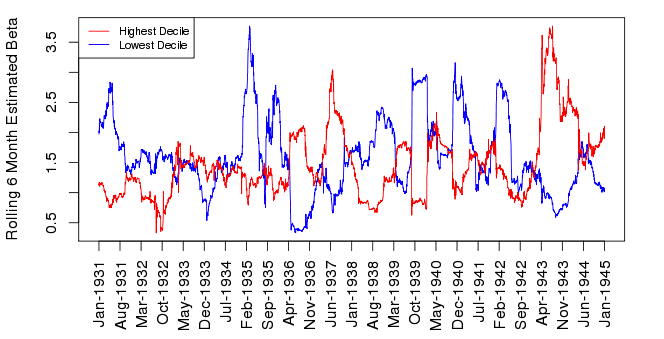
\includegraphics[scale=0.6]{betas1931.png}
\end{figure}

\begin{figure}[p]
\centering
\caption{\textbf{Momentum Market Beta for WML Portfolio 1931-1945.}}
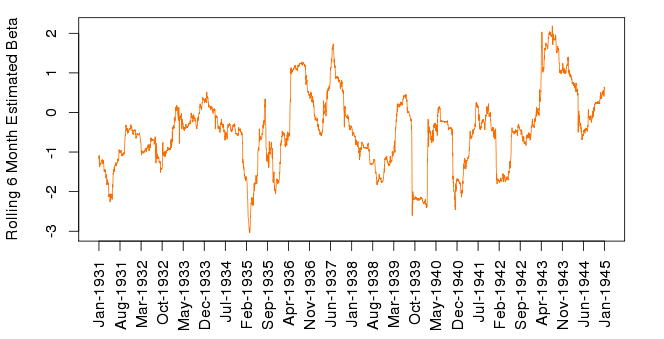
\includegraphics[scale=0.6]{betaWML1931.png}
\end{figure}

\begin{figure}[p]
\centering
\caption{\textbf{Momentum Market Betas of High10 and Low10 1999-2011.}}
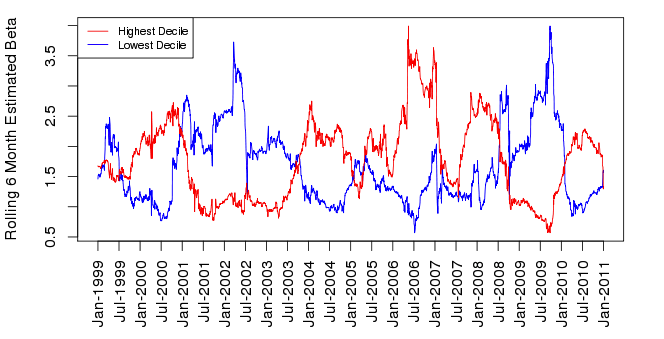
\includegraphics[scale=0.6]{betas1999.png}
\end{figure}

\begin{figure}[p]
\centering
\caption{\textbf{Momentum Market Beta for WML Portfolio 1999-2011.}}
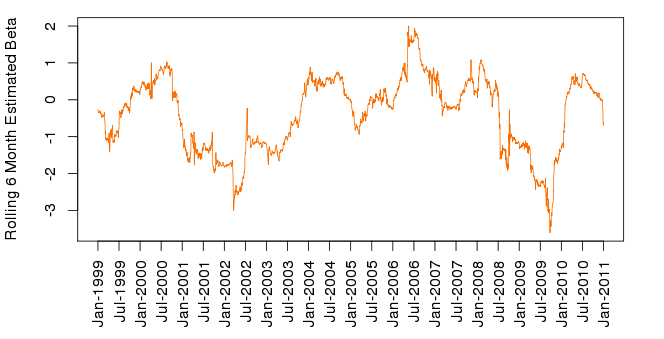
\includegraphics[scale=0.6]{betaWML1999.png}
\end{figure}

\subsection{The Effects of Bull and Bear Markets}

To investigate the magnitude of the effects that the market has on the changing beta of momentum portfolios, we construct a daily time series linear regression to predict the estimated market beta at time $t$. The form of the regression is shown in Equation 6. $\hat{\beta}^{*}_{i,t}$ is the estimated market beta calculated by Equation 5, and the market is defined as the same CRSP value-weighted index. The predictor is an indicator variable for whether or not the market during the two years leading up to time $t$ was bull or bear. Thus, $I_{B,t}$ is a 1 if the the cumulative market return at time $t$ for the past 504 days ($\approx 24$ months) was positive (i.e., a bull market), and 0 otherwise (i.e., a bear market). 
\begin{equation}
\beta_{i,t}^{*}=\alpha_{i}+\gamma_{i}*I_{B,t} + \epsilon_{t}
\end{equation}
Table 5 reports the results of the regression with respect to the High10, Low10, and WML portfolios for our sample of January 1926 through June 2013. We see that the coefficient for the bull/bear indicator is 0.355 for the High10 portfolio, meaning that when the cumulative returns of the CRSP value-weighted index for the past two years are positive, we expect the estimated market beta of the High10 portfolio to be 0.355 higher than it would be when the market return for the past two years is negative. The coefficient for the WML portfolio is also positive, at 0.913. On the other hand, the coefficient for the Low10 portfolio is negative at -0.579. All coefficients are significant at the 0.001 level.

\begin{table}[h]
\centering
\caption{\textbf{Point Estimates for Coefficients of Bull/Bear Indicator of Momentum Portfolios.}}
\begin{tabular}{l | c }
\hline
Portfolio $i$ & $\gamma_{i}$ \\
\hline
High10 & 0.335 \\
Low10 & -0.579 \\
WML & 0.913 \\
\end{tabular}
\end{table}

\subsection{Betas and Momentum Funds}

Up until now we have only examined how market swings affect our theoretical momentum portfolios. However, two of the momentum funds that we study have data that dates back to before the financial crisis of 2008, giving us an opportunity to examine the effects of a market crash on actual momentum portfolios. Returns for the RYAMX begin in June, 2005, while returns for the PowerShares DWA Momentum Portfolio ETF (PDP) begin in March, 2007.

We estimate the daily market betas for the RYAMX and PDP using 126 day rolling regressions as in Equation 5. Again, the market is defined as the CRSP value-weighted index. Figures 11 and 12 compare the estimated betas for the RYAMX and PDP with the estimated betas of the High10 portfolio. The black vertical line represents the market low-point of the time. 

\begin{figure}[p]
\caption{\textbf{Comparison of Market Betas for RYAMX and High10.}}
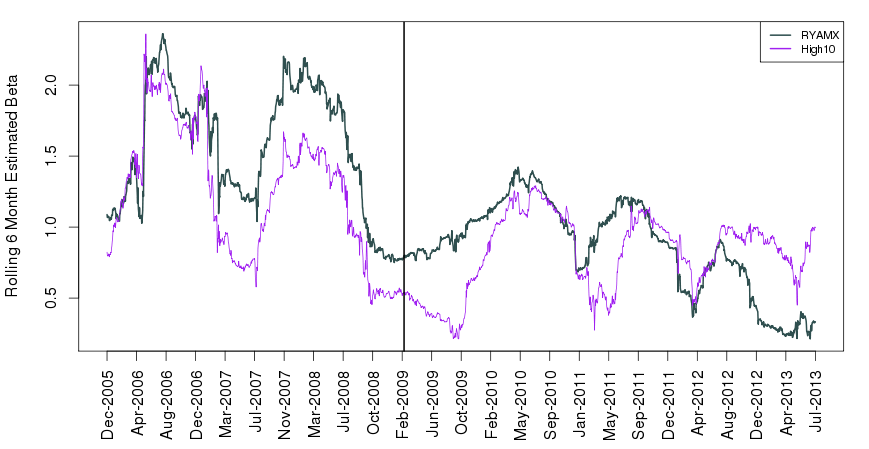
\includegraphics[scale=0.45]{RYAMXbetas.png}
\end{figure}

\begin{figure}[p]
\caption{\textbf{Comparison of Market Betas for PDP and High10.}}
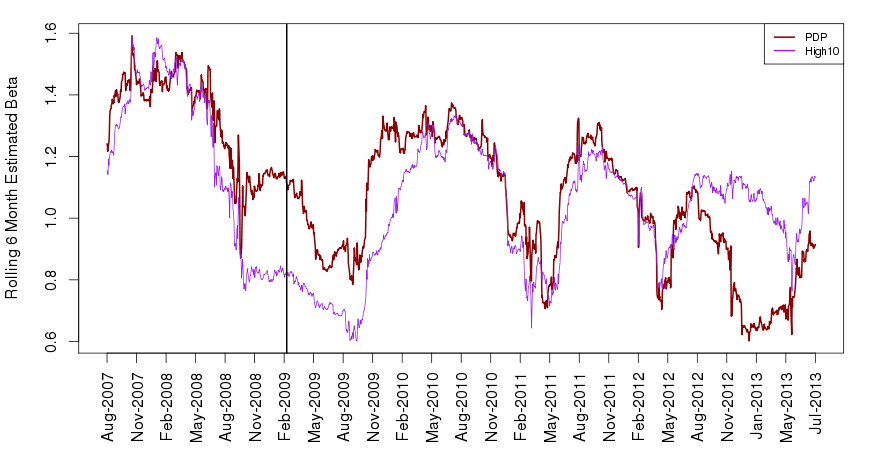
\includegraphics[scale=0.45]{PDPbetas.png}
\end{figure}

\begin{figure}[p]
\caption{\textbf{Comparison of Market Betas for AMOMX and High10.}}
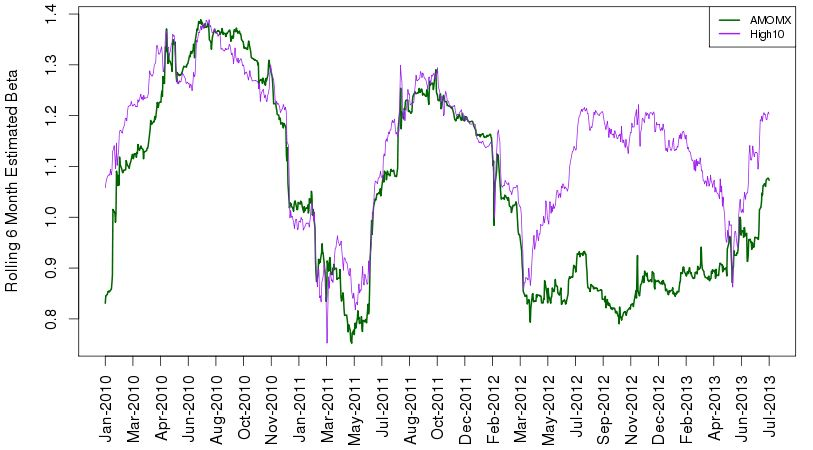
\includegraphics[scale=0.65]{AMOMXbetas.jpg}
\end{figure}

\begin{figure}[p]
\caption{\textbf{Comparison of Market Betas for BRSMX and High10.}}
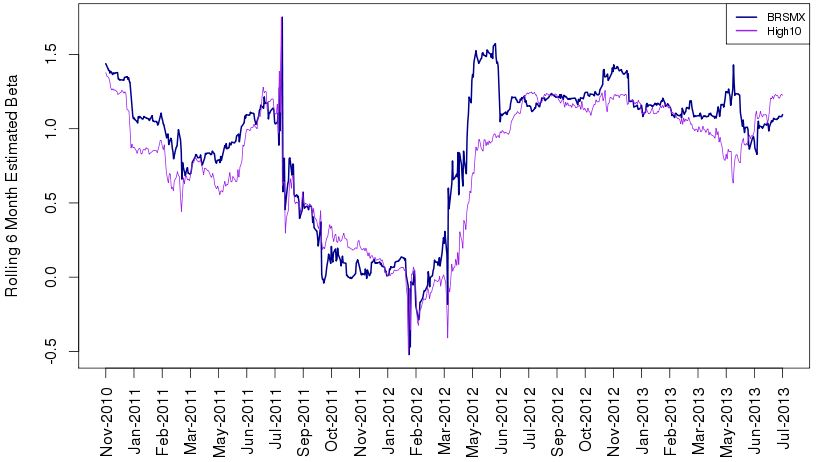
\includegraphics[scale=0.65]{BRSMXbetas.jpg}
\end{figure}

We notice that the betas for the RYAMX and PDP track the High10 betas closely, yet during the market's recovery following March 2009, they do not dip as low as the High10 betas. This suggests that managers may have hedged their bets in some way or altered their strategy slightly to buy some higher beta stocks during the recovery.

Figures 13 and 14 also show the estimated daily market betas of the AMOMX and BRSMX since the dates of their inception in 2010 to July 2013, compared to the estimated daily betas of the High10. As mentioned before, the betas for the AMOMX follow the High10 very closely up until March 2012, which is not surprising due to the explicit similarities between the strategies. The BRSMX also follows the High10 closely, suggesting that their strategy is primarily buy and hold the top momentum stocks, although all we can do is guess since the managers do not disclose their methods.

To quantify the difference in both expected return and market beta during bull and bear markets, we fit a conditional CAPM, shown in Equation 7, where $I_{B,t}$ interacts with $r_{m,t}$, the return of the market at time $t$. Again, $I_{B,t}$ is a 1 if the cumulative market return at time $t$ for the past 504 days was positive, and 0 otherwise. 
\begin{equation}
r_{i,t}=(\alpha_{i,0}+\alpha_{i,B}I_{B,t})+(\beta_{i,0}+\beta_{i,B}*I_{B,t})r_{m,t}+\epsilon_{t}
\end{equation}
Thus, the bull market alpha is $\alpha_{i,0}+\alpha_{i,B}$ and the bull market beta is $\beta_{i,0}+\beta_{i,B}$, while the bear market alpha and beta are just $\alpha_{i,0}$ and $\beta_{i,0}$. The results of this regression on the RYAMX and PDP are reported in Table 6.\footnote{The results of this regression were only significant for the RYAMX and PDP, not the AMOMX and BRSMX probably because we don't have enough historical data yet, since they have only been active since 2010.} For the RYAMX and PDP, the bull market beta is 0.177 and 0.128 higher, respectively, while the bear market alphas are -0.055 per day ($\approx$ -1.155 per month) and -0.092 per day ($\approx$ -1.932 per month). Our findings are consistent with the findings of GM and DM for the WML portfolio. They find that the bull market beta of WML portfolio is 1.2 higher, while the bear market alpha is -0.3\% per month.

\begin{table}[h]
\centering
\caption{\textbf{Coefficients of Conditional CAPM Regression.} \footnotesize{Regression is based on daily returns. T-statistics and p-values are reported under the point estimates of the coefficients.}}
\begin{tabular}{l | c | c | c | c }
\hline
Portfolio & $\alpha_{i,0}$ & $\alpha_{i,B}$ & $\beta_{i, 0}$ & $\beta_{i, B}$\\
\hline
RYAMX & -0.055 & 0.022 & 0.823 & 0.177 \\
 & -1.890 (0.059) & 0.672 (0.501) & 63.354 ($\approx$ 0) & 8.783 ($\approx$ 0)\\
\hline
PDP & -0.092 & 0.082 & 0.968 & 0.128\\
 & -3.507 ($\approx$ 0) & 2.651 ($\approx$ 0) & 83.448 ($\approx$ 0) & 6.828 ($\approx$ 0)\\
\end{tabular}
\end{table}

Equation 8 is used to determine whether the RYAMX and PDP exhibit the same optionality with regard to the market as the WML portfolio, which was analyzed by DM using this regression.\footnote{A similar regression was used by Henriksson and Merton (1981) for assessing the forecasting and market timing skills of money managers.} The $I_{R,t}$ term is now the bea$R$ market indicator, which is simply $1-I_{B}$, and $I_{U,t}$ is the $U$p-market indicator, which is a 1 if the contemporaneous return of the market on day $t$ was positive.
\begin{equation}
r_{i,t}=(\alpha_{i,0}+\alpha_{i,R}*I_{R,t})+[\beta_{i,0}+I_{R,t}(\beta_{i,R}+I_{U,t}*\beta_{i,R,U})]r_{m,t}+\epsilon_{t}.
\end{equation}
Thus, $\beta_{i,0}$ is the market beta of the portfolio during a bull market, $\beta_{i,0}+\beta_{i,R}$ is the market beta of the portfolio during a bear market when the contemporaneous return of the market is negative, and $\beta_{i,0}+\beta_{i,R}+\beta_{i,R,U}$ is the market beta during a bear market when the return of the market is positive. 

According to DM, the result of running this regression on the WML portfolio is a $B_{i,R,U}$ coefficient with a significantly negative value of $-0.814.$ Therefore, during bear market when the market return is positive, the point estimate of the portfolio beta is 0.814 lower than when the market return is negative. This means that ``the momentum portfolio is effectively short a call option on the market," DM note.

\begin{table}[t]
\centering
\caption{\textbf{Results of Regression 8.} \footnotesize{Regression is based on daily returns. T-statistics and p-values are reported under the point estimates of the coefficients.}}
\begin{tabular}{l | c | c | c | c | c }
\hline
Portfolio & $\alpha_{i,0}$ & $\alpha_{i,R}$ & $\beta_{i,0}$ & $\beta_{i,R}$ & $\beta_{i,R,U}$\\
\hline
RYAMX & -0.033 & 0.133 & 1.000 & -0.080 & -0.200 \\
 & -2.113 (0.035) & 3.085 (0.002) & 65.078 ($\approx$ 0) & -2.999 (0.003) & -5.591 ($\approx$ 0) \\
\hline
PDP & -0.010 & 0.147 & 1.096 & 0.016 & -0.294 \\
 & -0.615 (0.538) & 3.804 ($\approx$ 0) & 76.554 ($\approx$ 0) & 0.679 (0.497) & -9.404 ($\approx$ 0)\\
\end{tabular}
\end{table}

Table 7 reports the results of the regression on the RYAMX and PDP. We find that the $\beta_{i,R,U}$ term is significantly negative for both portfolios, meaning that they exhibit the same optionality with regard to the market as the WML portfolio.\footnote{Unlike DM, we use daily returns instead of monthly, however this should not affect the results.} The fact that these coefficients for the RYAMX and PDP are not as great in magnitude as that of WML is probably due to the fact that this option-like behavior is driven by the losing stocks, as found by DM, and we have strong evidence that the strategies of the RYAMX and PDP are mostly to go long the winners.

\section{Conclusion and Future Studies} %%%%%%%%%%%%%%%%%%%%%%%%%%%%%%%%%%

Previous studies on momentum have all lacked the necessary consideration of transaction costs, and hence have concluded that momentum investing leads to abnormal returns. Thus momentum has often been cited as a counter-example to market efficiency. Yet after examining real momentum funds, we find the results to be quite different. The four momentum funds we have studied have all substantially underperformed the market. 

While it seems that transaction costs are the primary cause for the meager performance, the changing betas of the RYAMX and PDP also give us clues as to why they have performed so poorly. We find that following a market decline, these funds are essentially short a call option on the market.

While our results are all statistically significant, this is not to be the final word on momentum. Further studies of these same funds in different economic conditions may yield different results. It also remains to be seen what the exact transactions costs are and how the strategies between funds differ. Perhaps strategies with different holding and formation periods will be able to beat the market when others fail.


%%%%%%%%%%%%%%%%%%%%%%%%%%%%%%%%%%%%%%%%%%%%%%%%%%%
\newpage \begin{thebibliography}{100} %%%%%%%%%%%%%%%%%%%%%%%%%

\bibitem{A} Asness, Clifford, 1994, Variables that explain stock returns, University of Chicago Ph.D dissertation.

\bibitem{ALS} Asness, Clifford, John Liew, and Ross Stevens, 1997, Parallels between the cross-sectional predictability of stock and country returns, \emph{The Journal of Portfolio Management} Vol. 23, No. 3, 79-87.

\bibitem{AMP} Asness, Clifford, Tobias Moskowitz, and Lasse Pedersen, 2008, Value and momentum everywhere, University of Chicago working paper.

\bibitem{C} Carhart, Mark, 1997, On persistence in mutual fund performance, \emph{The Journal of Finance} Vol. 52, 57-82.

\bibitem{DM} Daniel, Kent and Tobias Moskowitz, 2011, Momentum crashes, University of Chicago, Columbia University working paper.

\bibitem{DT} DeBondt, Werner and Richard Thaler, 1985, Does the stock market overreact? \emph{The Journal of Finance} Vol. 40, No. 3, 793-805.

\bibitem{F} Fama, Eugene, 1991, Efficient capital markets: II, \emph{The Journal of Finance} Vol. 46, No. 5, 1575-1617.

\bibitem{FF} Fama, Eugene and Kenneth French, 1992, The cross-section of expected stock returns, \emph{The Journal of Finance} Vol. 47, No. 2, 427-465.

\bibitem{FF2} \underline{\hspace{1cm}}, 1996, Multifactor explanations of asset pricing anomalies, \emph{The Journal of Finance} Vol. 51, No. 1, 55-84.

\bibitem{FF3} \underline{\hspace{1cm}}, 2010, Size, value, and momentum in international stock returns, University of Chicago and Dartmouth College working paper.

\bibitem{FIM} Frazzini, Andrea, Ronen Israel, and Tobias Moskowitz, 2012, Trading costs of asset pricing anomalies. University of Chicago working paper.

\bibitem{GHR} Gorton, Gary, Fumio Hayashi, and K. Geert Rouwenhorst, 2007, The fundamentals of commodity futures returns, University of Pennsylvania working paper.

\bibitem{GM} Grinblatt, Mark and Tobias Moskowitz, 1999, Do industries explain momentum? \emph{The Journal of Finance} Vol. 54, 1249-1290.

\bibitem{GM2} \underline{\hspace{1cm}}, 2004, Predicting stock price movements from past returns: the role of consistency and tax-loss selling, \emph{The Journal of Financial Economics} Vol. 71, 541-579.

\bibitem{GrundM} Grundy, Bruce and Spencer Martin, 2001, Understanding the nature of the risks and the source of the rewards to momentum investing, \emph{Review of Financial Studies} Vol. 14, 29-78.

\bibitem{HB} Haugen, Robert and Nardin Baker, 2010, Case closed. \emph{The Handbook of Portfolio Construction: Contemporary Applications of Markowitz Techniques} 601-619.

\bibitem{HM} Henriksson, Roy, and Robert Merton, 1981, On market timing and investment performance. II. Statistical procedures for evaluating and forecasting skills, \emph{The Journal of Business} Vol. 54, 513-533.

\bibitem{IM} Israel, Ronen and Tobias Moskowitz, 2011, How tax efficient are equity styles? University of Chicago working paper.

\bibitem{J} Jagedeesh, Narasimhan, 1990, Evidence of predictable behavior of security returns, \emph{The Journal of Finance} Vol. 45, No. 3, 881-898.

\bibitem{JT} Jegadeesh, Narasimhan and Sheridan Titman, 1993, Returns to buying winners and selling losers: implications for stock market efficiency. \emph{The Journal of Finance} Vol. 48, 64-91.

\bibitem{Le} LeBaron, Blake, 1999, Technical trading rules profitability and foreign exchange intervention, \emph{The Journal of International Economics} Vol. 49, 125-143.

\bibitem{L} Lehmann, Bruce, 1990, Fads, martingales and market efficiency, \emph{The Quarterly Journal of Economics} Vol. 105, 1-28.

\bibitem{LSZ} Lesmond, David, Michael Schill, and Chunsheng Zhou, 2004, The illusory nature of momentum profits, \emph{The Journal of Financial Economics} Vol. 71, 349-380.

\bibitem{LBM} Li, Xiafei, Chris Brooks, and Joelle Miffre, 2009, Transaction costs, trading volume, and momentum strategies, working paper.

\bibitem{LM} Lo, Andrew, and Craig MacKinaly, 1990, When are contrarian profits due to stock market overreaction? \emph{The Review of Financial Studies} Vol. 3, No. 3, 175-205.

\end{thebibliography}

\end{document}